\begin{frame}
\titlepage
\end{frame}

\begin{frame}{This lecture}
\vspace*{1cm}
\begin{itemize}
       \item Encoder-Decoder
       \item Attention 
       \item Their applications in NLP
\end{itemize}
\end{frame}
%%%%%%%%%%%%%%%%%%%%%%%%%%%%%%%%

\begin{frame}{Encoder}

     A neural model to transform a text into a vector in an embedding space.
\begin{center}
        
        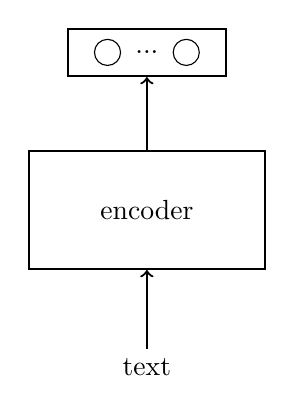
\begin{tikzpicture}
            \node(text) at (0,0) [] {text};
            \node(encoder) at (0,2) [draw, minimum width=3cm, minimum height=1.5cm, thick] {encoder};
            \node(enc_out1) at (-0.5,4) [draw,circle] {};
            \node(enc_out2) at (0.0,4) [] {...};
            \node(enc_out3) at (0.5,4) [draw,circle] {};
            \node(enc_out_box) at (0.0,4) [draw,minimum width=2cm, minimum height=0.6cm, thick] {};
            
            \draw[->, thick] (text) -- (encoder);
            \draw[->, thick] (encoder) -- (enc_out_box);
        \end{tikzpicture}
\end{center}

Different types of neural encoders are
\begin{itemize}
    \item pretrained word embeddings
    \item MLPs, CNNs, RNNs, Transformers, ...
\end{itemize}
\end{frame}

\begin{frame}{Decoder}
         A neural model to transform a vector from an embedding space to a text.
\begin{center}
        
        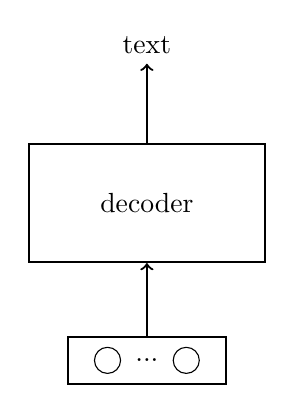
\begin{tikzpicture}
            \node(dec_in1) at (-0.5,0) [draw,circle] {};
            \node(dec_in2) at (0.0,0) [] {...};
            \node(dec_in3) at (0.5,0) [draw,circle] {};
            \node(dec_in_box) at (0.0,0) [draw,minimum width=2cm, minimum height=0.6cm, thick] {};
            
            \node(decoder) at (0,2) [draw, minimum width=3cm, minimum height=1.5cm, thick] {decoder};
            \node(text) at (0,4) [] {text};
            
            \draw[->, thick] (dec_in_box) -- (decoder);
            \draw[->, thick] (decoder) -- (text);
        \end{tikzpicture}
\end{center}
Different types of language models can be used as decoders
\begin{itemize}
    \item RNN-based LMs
    \item Transformer-based LMs
\end{itemize}
\end{frame}

\begin{frame}{Encoder-Decoder}
\begin{center}
\scalebox{0.8}{

        
        \begin{tikzpicture}
            \node(inp_text) at (0,0) [] {input text};
            \node(encoder) at (0,2) [draw, minimum width=2cm, minimum height=1.5cm, thick] {encoder};
            \node(enc_out1) at (-0.5,4) [draw,circle] {};
            \node(enc_out2) at (0.0,4) [] {...};
            \node(enc_out3) at (0.5,4) [draw,circle] {};
            \node(enc_out_box) at (0,4) [draw,minimum width=2cm, minimum height=0.6cm, thick] {};
            
            \draw[->, thick] (inp_text) -- (encoder);
            \draw[->, thick] (encoder) -- (enc_out_box);
            
        
            \node(decoder) at (0,6) [draw, minimum width=2cm, minimum height=1.5cm, thick] {decoder};
            \node(out_text) at (0,8) [] {output text};
            
            \draw[->, thick] (enc_out_box) -- (decoder);
            \draw[->, thick] (decoder) -- (out_text);
            
            \overlay<2->{
            \node(enc_out1) at (2.5,4) [myblue] {context vector };
            }
            
        \end{tikzpicture}
}
\end{center}
     
\end{frame}

\begin{frame}{RNN Encoder}
\centering
\vspace{2cm}
\begin{tikzpicture}
            \tikzset{layer/.style={draw,rectangle, fill=gray!20, thick}}
            \tikzset{edge/.style={->, thick}}
        
            \node(x1) at (0,0) [layer, minimum width=1cm] {$\bm{x_1}$};
            \node(h1) at (0,1.5) [layer, minimum width=0.5cm] {$\bm{h_1}$};
            \draw[edge](x1) --  (h1);
            
        

            \node(x2) at (2,0) [layer, minimum width=1cm] {$\bm{x_2}$};
            \node(h2) at (2,1.5) [layer, minimum width=0.5cm] {$\bm{h_2}$};
            \draw[edge](x2) --  (h2);
            
        
            \node(x3) at (4,0) [layer, minimum width=1cm] {$\bm{x_3}$};
            \node(h3) at (4,1.5) [layer, minimum width=0.5cm] {$\bm{h_3}$};
            \draw[edge](x3) -- (h3);
            
            \draw[edge, myblue] (h1) -- (h2);
            \draw[edge,myblue] (h2) --  (h3);


            \node(end_out1) at (1.5,3) [draw,circle] {};
            \node(end_out2) at (2.0,3) [] {...};
            \node(end_out3) at (2.5,3) [draw,circle] {};
            \node(end_out_box) at (2.0,3) [draw,minimum width=2cm, minimum height=0.6cm, thick] {};
            \draw[edge] (h3) -- (end_out_box);

        \end{tikzpicture}
\end{frame}

\begin{frame}{RNN Decoder}
\centering
\vspace{2cm}
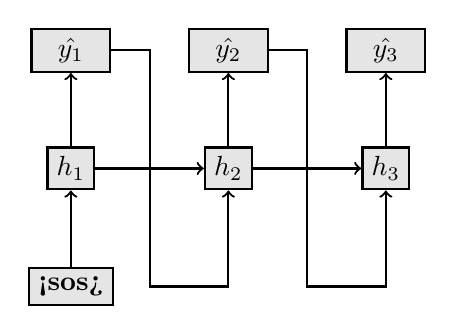
\begin{tikzpicture}
            \tikzset{layer/.style={draw,rectangle, fill=gray!20, thick}}
            \tikzset{edge/.style={->, thick}}


            % \node(dec1) at (9.5,0) [draw,circle] {};
            % \node(dec2) at (10.0,0) [] {...};
            % \node(dec3) at (10.5,0) [draw,circle] {};
            % \node(dec_box) at (10.0,0) [draw,minimum width=2cm, minimum height=0.6cm, thick] {};
    
            \node(x1) at (8,1.5) [layer, minimum width=1cm] {\textbf{<sos>}};
            \node(h1) at (8,3) [layer, minimum width=0.5cm] {$\bm{h_1}$};
            \draw[edge](x1) --  (h1);
            \node(y1_hat) at (8,4.5) [layer, minimum width=1cm] {$\bm{\hat{y_1}}$};
            \draw[edge](h1) --  (y1_hat);
            
    
            %\node(x2) at (10,1.5) [layer, minimum width=1cm] {};
            \node(h2) at (10,3) [layer, minimum width=0.5cm] {$\bm{h_2}$};
            %\draw[edge](x2) --  (h2);
            \node(y2_hat) at (10,4.5) [layer, minimum width=1cm] {$\bm{\hat{y_2}}$};
            \draw[edge](h2) --  (y2_hat);
            \draw[edge](y1_hat) -- (9,4.5) -- (9,1.5) -- (10,1.5) -- (h2);
            
            %\node(x3) at (12,1.5) [layer, minimum width=1cm] {$\bm{x_3}$};
            \node(h3) at (12,3) [layer, minimum width=0.5cm] {$\bm{h_3}$};
            %\draw[edge](x3) -- (h3);
            \node(y3_hat) at (12,4.5) [layer, minimum width=1cm] {$\bm{\hat{y_3}}$};
            \draw[edge](h3) --  (y3_hat);
            \draw[edge](y2_hat) -- (11,4.5) -- (11,1.5) -- (12,1.5) -- (h3);


            
            \draw[edge] (h1) -- (h2);
            \draw[edge] (h2) --  (h3);
            % \draw[edge] (dec_box)-- (h1);
        
        \end{tikzpicture}
\end{frame}

\begin{frame}{RNN-based Encoder-Decoder}
\centering
\scalebox{0.8}{
    \begin{tikzpicture}
            \tikzset{layer/.style={draw,rectangle, fill=gray!20, thick}}
            \tikzset{edge/.style={->, thick}}
        
            \node(x1) at (0,0) [layer, minimum width=1cm] {$\bm{x_1}$};
            \node(enc_h1) at (0,1.5) [layer, minimum width=0.5cm] {$\bm{h^e_1}$};
            \draw[edge](x1) --  (enc_h1);
            
        

            \node(x2) at (2,0) [layer, minimum width=1cm] {$\bm{x_2}$};
            \node(enc_h2) at (2,1.5) [layer, minimum width=0.5cm] {$\bm{h^e_2}$};
            \draw[edge](x2) --  (enc_h2);
            
        
            \node(x3) at (4,0) [layer, minimum width=1cm] {$\bm{x_3}$};
            \node(enc_h3) at (4,1.5) [layer, minimum width=0.5cm] {$\bm{h^e_3}$};
            \draw[edge](x3) -- (enc_h3);
            
            \draw[edge] (enc_h1) -- (enc_h2);
            \draw[edge] (enc_h2) --  (enc_h3);


            \node(enc_out1) at (1.5,3) [draw,circle] {};
            \node(enc_out2) at (2.0,3) [] {...};
            \node(enc_out3) at (2.5,3) [draw,circle] {};
            \node(enc_out_box) at (2.0,3) [draw,minimum width=2cm, minimum height=0.6cm, thick] {};
            \draw[edge] (enc_h3) --  (enc_out_box);

            \node(sos) at (0,4.5) [layer, minimum width=1cm] {\textbf{<sos>}};
            \node(dec_h1) at (0,6.0) [layer, minimum width=0.5cm] {$\bm{h^d_1}$};
            \node(y1_hat) at (0,7.5) [layer, minimum width=1cm] {$\bm{\hat{y_1}}$};
            \draw[edge](sos) --  (dec_h1);
            \draw[edge](dec_h1) --  (y1_hat);
            \draw[edge,myblue, bend left=30](enc_out_box) edge  (dec_h1);
                
            \node(dec_h2) at (2,6.0) [layer, minimum width=0.5cm] {$\bm{h^d_2}$};
            \node(y2_hat) at (2,7.5) [layer, minimum width=1cm] {$\bm{\hat{y_2}}$};
            \draw[edge](dec_h2) --  (y2_hat);
            \draw[edge](y1_hat) -- (1,7.5) -- (1,5.0) -- (2,5.0) -- (dec_h2);
            %\draw[edge,myblue, bend left=30](enc_out_box) edge  (dec_h2);
                        
            \node(dec_h3) at (4,6.0) [layer, minimum width=0.5cm] {$\bm{h^d_3}$};
            \node(y3_hat) at (4,7.5) [layer, minimum width=1cm] {$\bm{\hat{y_3}}$};
            \draw[edge](dec_h3) --  (y3_hat);
            \draw[edge](y2_hat) -- (3,7.5) -- (3,5) -- (4,5) -- (dec_h3);

        \end{tikzpicture}
        }
\end{frame}


\begin{frame}{RNN-based Encoder-Decoder}
    \begin{itemize}
        \item The context vector is used to  initialize the hidden state of the decoder. 
        \item Its impact vanishes at the last steps of the decoder. 
    \end{itemize}
\end{frame}


\begin{frame}{RNN-based Encoder-Decoder}
\centering
\scalebox{0.8}{
    \begin{tikzpicture}
            \tikzset{layer/.style={draw,rectangle, fill=gray!20, thick}}
            \tikzset{edge/.style={->, thick}}
        
            \node(x1) at (0,0) [layer, minimum width=1cm] {$\bm{x_1}$};
            \node(enc_h1) at (0,1.5) [layer, minimum width=0.5cm] {$\bm{h^e_1}$};
            \draw[edge](x1) --  (enc_h1);
            
        

            \node(x2) at (2,0) [layer, minimum width=1cm] {$\bm{x_2}$};
            \node(enc_h2) at (2,1.5) [layer, minimum width=0.5cm] {$\bm{h^e_2}$};
            \draw[edge](x2) --  (enc_h2);
            
        
            \node(x3) at (4,0) [layer, minimum width=1cm] {$\bm{x_3}$};
            \node(enc_h3) at (4,1.5) [layer, minimum width=0.5cm] {$\bm{h^e_3}$};
            \draw[edge](x3) -- (enc_h3);
            
            \draw[edge] (enc_h1) -- (enc_h2);
            \draw[edge] (enc_h2) --  (enc_h3);


            \node(enc_out1) at (1.5,3) [draw,circle] {};
            \node(enc_out2) at (2.0,3) [] {...};
            \node(enc_out3) at (2.5,3) [draw,circle] {};
            \node(enc_out_box) at (2.0,3) [draw,minimum width=2cm, minimum height=0.6cm, thick] {};
            \draw[edge] (enc_h3) --  (enc_out_box);

            \node(sos) at (0,4.5) [layer, minimum width=1cm] {\textbf{<sos>}};
            \node(dec_h1) at (0,6.0) [layer, minimum width=0.5cm] {$\bm{h^d_1}$};
            \node(y1_hat) at (0,7.5) [layer, minimum width=1cm] {$\bm{\hat{y_1}}$};
            \draw[edge](sos) --  (dec_h1);
            \draw[edge](dec_h1) --  (y1_hat);
            \draw[edge,myblue, bend left=30](enc_out_box) edge  (dec_h1);
                
            \node(dec_h2) at (2,6.0) [layer, minimum width=0.5cm] {$\bm{h^d_2}$};
            \node(y2_hat) at (2,7.5) [layer, minimum width=1cm] {$\bm{\hat{y_2}}$};
            \draw[edge](dec_h2) --  (y2_hat);
            \draw[edge](y1_hat) -- (1,7.5) -- (1,5.0) -- (2,5.0) -- (dec_h2);
            \draw[edge,myblue, bend left=30](enc_out_box) edge  (dec_h2);
                        
            \node(dec_h3) at (4,6.0) [layer, minimum width=0.5cm] {$\bm{h^d_3}$};
            \node(y3_hat) at (4,7.5) [layer, minimum width=1cm] {$\bm{\hat{y_3}}$};
            \draw[edge](dec_h3) --  (y3_hat);
            \draw[edge](y2_hat) -- (3,7.5) -- (3,5) -- (4,5) -- (dec_h3);
            \draw[edge,myblue, bend left=30](enc_out_box) edge  (dec_h3);
            
        \end{tikzpicture}
}
\end{frame}


% \begin{frame}{RNN-based Encoder-Decoder}
% \vspace{2cm}
% \scalebox{0.8}{
%     \begin{tikzpicture}
%             \tikzset{layer/.style={draw,rectangle, fill=gray!20, thick}}
%             \tikzset{edge/.style={->, thick}}
        
%             \node(x1) at (0,0) [layer, minimum width=1cm] {$\bm{x_1}$};
%             \node(h1) at (0,1.5) [layer, minimum width=0.5cm] {$\bm{h_1}$};
%             \draw[edge](x1) --  (h1);
            
        

%             \node(x2) at (2,0) [layer, minimum width=1cm] {$\bm{x_2}$};
%             \node(h2) at (2,1.5) [layer, minimum width=0.5cm] {$\bm{h_2}$};
%             \draw[edge](x2) --  (h2);
            
        
%             \node(x3) at (4,0) [layer, minimum width=1cm] {$\bm{x_3}$};
%             \node(h3) at (4,1.5) [layer, minimum width=0.5cm] {$\bm{h_3}$};
%             \draw[edge](x3) -- (h3);
            
%             \draw[edge, myblue] (h1) -- (h2);
%             \draw[edge,myblue] (h2) --  (h3);


%             \node(end_out1) at (5,3) [draw,circle] {};
%             \node(end_out2) at (5.5,3) [] {...};
%             \node(end_out3) at (6.0,3) [draw,circle] {};
%             \node(end_out_box) at (5.5,3) [draw,minimum width=2cm, minimum height=0.6cm, thick] {};
%             \draw[edge] (h3) -- (5.5,1.5);
%             \draw[edge] (5.5, 1.5) -- (end_out_box);


%             \node(dec1) at (5,3) [draw,circle] {};
%             \node(dec2) at (5.5,3) [] {...};
%             \node(dec3) at (6.0,3) [draw,circle] {};
%             \node(dec_box) at (5.5,3) [draw,minimum width=2cm, minimum height=0.6cm, thick] {};
    
%             \node(x1) at (8,1.5) [layer, minimum width=1cm] {\textbf{<sos>}};
%             \node(h1) at (8,3) [layer, minimum width=0.5cm] {$\bm{h_1}$};
%             \draw[edge](x1) --  (h1);
%             \node(y1_hat) at (8,4.5) [layer, minimum width=1cm] {$\bm{\hat{y_1}}$};
%             \draw[edge](h1) --  (y1_hat);
            
%             \node(h2) at (10,3) [layer, minimum width=0.5cm] {$\bm{h_2}$};
%             \node(y2_hat) at (10,4.5) [layer, minimum width=1cm] {$\bm{\hat{y_2}}$};
%             \draw[edge](h2) --  (y2_hat);
%             \draw[edge](y1_hat) -- (9,4.5) -- (9,1.5) -- (10,1.5) -- (h2);
            
%             %\node(x3) at (12,1.5) [layer, minimum width=1cm] {$\bm{x_3}$};
%             \node(h3) at (12,3) [layer, minimum width=0.5cm] {$\bm{h_3}$};
%             %\draw[edge](x3) -- (h3);
%             \node(y3_hat) at (12,4.5) [layer, minimum width=1cm] {$\bm{\hat{y_3}}$};
%             \draw[edge](h3) --  (y3_hat);
%             \draw[edge](y2_hat) -- (11,4.5) -- (11,1.5) -- (12,1.5) -- (h3);

%             \draw[edge, myblue] (end_out_box) edge (y1_hat);
%             \draw[edge, myblue] (end_out_box) edge (y2_hat);
%             \draw[edge, myblue] (end_out_box) edge (y3_hat);
            
%             \draw[edge] (h1) -- (h2);
%             \draw[edge] (h2) --  (h3);
%             \draw[edge] (dec_box)-- (h1);
%         \end{tikzpicture}
%         }
% \end{frame}



\begin{frame}{RNN-based Encoder-Decoder}
\begin{itemize}
    \item The output of the encoder is known as the context vector.
    \item The dimensionality of the context vector is fixed. 
    \item However, different input texts might have different length. 
    \item So, considering the hidden state of the RNN encoder may not capture the entire input text.
    \item This is a problem  especially for long input texts. 
    % \item The other problem is that context vector is fixed for all decoding steps
    % \item However, at any decoding step, it might be more informative to focus on a subset of words in the input sentence
\end{itemize}
\end{frame}

\begin{frame}{RNN-based Encoder-Decoder}
\centering
\scalebox{0.8}{
    \begin{tikzpicture}
            \tikzset{layer/.style={draw,rectangle, fill=gray!20, thick}}
            \tikzset{edge/.style={->, thick}}
        
            \node(x1) at (0,0) [layer, minimum width=1cm] {$\bm{x_1}$};
            \node(enc_h1) at (0,1.5) [layer, minimum width=0.5cm] {$\bm{h^e_1}$};
            \draw[edge](x1) --  (enc_h1);
            
        

            \node(x2) at (2,0) [layer, minimum width=1cm] {$\bm{x_2}$};
            \node(enc_h2) at (2,1.5) [layer, minimum width=0.5cm] {$\bm{h^e_2}$};
            \draw[edge](x2) --  (enc_h2);
            
        
            \node(x3) at (4,0) [layer, minimum width=1cm] {$\bm{x_3}$};
            \node(enc_h3) at (4,1.5) [layer, minimum width=0.5cm] {$\bm{h^e_3}$};
            \draw[edge](x3) -- (enc_h3);
            
            \draw[edge] (enc_h1) -- (enc_h2);
            \draw[edge] (enc_h2) --  (enc_h3);


            \node(sum) at (2,3) [myblue]{$\bigoplus$};
            \node(context_vec) at (2.0,4.0) [layer, minimum width=1cm]{\textcolor{myblue}{$c$}};
            \draw[myblue, edge] (enc_h1) edge (sum);
            \draw[myblue, edge] (enc_h2) edge (sum);
            \draw[myblue, edge] (enc_h3) edge (sum);
            \draw[myblue, edge] (sum) edge (context_vec);
            
            

            % \node(enc_out1) at (1.5,3) [draw,circle] {};
            % \node(enc_out2) at (2.0,3) [] {...};
            % \node(enc_out3) at (2.5,3) [draw,circle] {};
            % \node(enc_out_box) at (2.0,3) [draw,minimum width=2cm, minimum height=0.6cm, thick] {};
            % \draw[edge] (enc_h3) --  (enc_out_box);




            \node(sos) at (0,4.5) [layer, minimum width=1cm] {\textbf{<sos>}};
            \node(dec_h1) at (0,6.0) [layer, minimum width=0.5cm] {$\bm{h^d_1}$};
            \node(y1_hat) at (0,7.5) [layer, minimum width=1cm] {$\bm{\hat{y_1}}$};
            \draw[edge](sos) --  (dec_h1);
            \draw[edge](dec_h1) --  (y1_hat);
            \draw[edge,myblue, bend left=30](context_vec) edge  (dec_h1);
                
            \node(dec_h2) at (2,6.0) [layer, minimum width=0.5cm] {$\bm{h^d_2}$};
            \node(y2_hat) at (2,7.5) [layer, minimum width=1cm] {$\bm{\hat{y_2}}$};
            \draw[edge](dec_h2) --  (y2_hat);
            \draw[edge](y1_hat) -- (1,7.5) -- (1,5.0) -- (2,5.0) -- (dec_h2);
            \draw[edge,myblue, bend left=30](context_vec) edge  (dec_h2);
                        
            \node(dec_h3) at (4,6.0) [layer, minimum width=0.5cm] {$\bm{h^d_3}$};
            \node(y3_hat) at (4,7.5) [layer, minimum width=1cm] {$\bm{\hat{y_3}}$};
            \draw[edge](dec_h3) --  (y3_hat);
            \draw[edge](y2_hat) -- (3,7.5) -- (3,5) -- (4,5) -- (dec_h3);
            \draw[edge,myblue, bend left=30](context_vec) edge  (dec_h3);
            
        \end{tikzpicture}
}
\end{frame}


% \begin{frame}{Mean Context}
% \vspace{2cm}
% \scalebox{0.8}{
%     \begin{tikzpicture}
%             \tikzset{layer/.style={draw,rectangle, fill=gray!20, thick}}
%             \tikzset{edge/.style={->, thick}}
        
%             \node(x1) at (0,0) [layer, minimum width=1cm] {$\bm{x_1}$};
%             \node(h1) at (0,1.5) [layer, minimum width=0.5cm] {$\bm{h_1}$};
%             \draw[edge](x1) --  (h1);
            
        

%             \node(x2) at (2,0) [layer, minimum width=1cm] {$\bm{x_2}$};
%             \node(h2) at (2,1.5) [layer, minimum width=0.5cm] {$\bm{h_2}$};
%             \draw[edge](x2) --  (h2);
            
        
%             \node(x3) at (4,0) [layer, minimum width=1cm] {$\bm{x_3}$};
%             \node(h3) at (4,1.5) [layer, minimum width=0.5cm] {$\bm{h_3}$};
%             \draw[edge](x3) -- (h3);
            
%             \draw[edge] (h1) -- (h2);
%             \draw[edge] (h2) --  (h3);



%             \node(enc_out1) at (5,3) [draw,circle] {};
%             \node(enc_out2) at (5.5,3) [] {...};
%             \node(enc_out3) at (6.0,3) [draw,circle] {};
%             \node(enc_out_box) at (5.5,3) [draw,minimum width=2cm, minimum height=0.6cm, thick] {};
            
%             \node(mean) at (2,3) [draw,circle,myblue] {Mean};
%             \draw[edge,myblue] (h1) -- (mean);
%             \draw[edge,myblue] (h2) -- (mean);
%             \draw[edge,myblue] (h3) -- (mean);
%             \draw[edge,myblue] (mean) -- (enc_out_box);


%             \node(dec1) at (5,3) [draw,circle] {};
%             \node(dec2) at (5.5,3) [] {...};
%             \node(dec3) at (6.0,3) [draw,circle] {};
%             \node(dec_box) at (5.5,3) [draw,minimum width=2cm, minimum height=0.6cm, thick] {};
    
%             \node(x1) at (8,1.5) [layer, minimum width=1cm] {\textbf{<sos>}};
%             \node(h1) at (8,3) [layer, minimum width=0.5cm] {$\bm{h_1}$};
%             \draw[edge](x1) --  (h1);
%             \node(y1_hat) at (8,4.5) [layer, minimum width=1cm] {$\bm{\hat{y_1}}$};
%             \draw[edge](h1) --  (y1_hat);
            
%             \node(h2) at (10,3) [layer, minimum width=0.5cm] {$\bm{h_2}$};
%             \node(y2_hat) at (10,4.5) [layer, minimum width=1cm] {$\bm{\hat{y_2}}$};
%             \draw[edge](h2) --  (y2_hat);
%             \draw[edge](y1_hat) -- (9,4.5) -- (9,1.5) -- (10,1.5) -- (h2);
            
%             %\node(x3) at (12,1.5) [layer, minimum width=1cm] {$\bm{x_3}$};
%             \node(h3) at (12,3) [layer, minimum width=0.5cm] {$\bm{h_3}$};
%             %\draw[edge](x3) -- (h3);
%             \node(y3_hat) at (12,4.5) [layer, minimum width=1cm] {$\bm{\hat{y_3}}$};
%             \draw[edge](h3) --  (y3_hat);
%             \draw[edge](y2_hat) -- (11,4.5) -- (11,1.5) -- (12,1.5) -- (h3);


            
%             \draw[edge] (h1) -- (h2);
%             \draw[edge] (h2) --  (h3);
%             \draw[edge] (dec_box)-- (h1);
%         \end{tikzpicture}
%         }
% \end{frame}


\begin{frame}{RNN-based Encoder-Decoder}
\begin{itemize}
    \item The other problem is that context vector is unique for all decoding steps.
    \item The encoder treats all tokens of the input sentence equally important to produce a context vector. 
    \item However, at any decoding step, the decoder should focus on tokens of the input sentence differently. 
\end{itemize}
\end{frame}


\begin{frame}{Attention}
\centering


    \begin{tikzpicture}
            \tikzset{layer/.style={draw,rectangle, fill=gray!20, thick}}
            \tikzset{edge/.style={->, thick}}
        
            \node(x1) at (0,0) [layer, minimum width=1cm] {$\bm{x_1}$};
            \node(enc_h1) at (0,1.5) [layer, minimum width=0.5cm] {$\bm{h^e_1}$};
            \draw[edge](x1) --  (enc_h1);
            

            \node(x2) at (2,0) [layer, minimum width=1cm] {$\bm{x_2}$};
            \node(enc_h2) at (2,1.5) [layer, minimum width=0.5cm] {$\bm{h^e_2}$};
            \draw[edge](x2) --  (enc_h2);
            
        
            \node(x3) at (4,0) [layer, minimum width=1cm] {$\bm{x_3}$};
            \node(enc_h3) at (4,1.5) [layer, minimum width=0.5cm] {$\bm{h^e_3}$};
            \draw[edge](x3) -- (enc_h3);
            
            \draw[edge] (enc_h1) -- (enc_h2);
            \draw[edge] (enc_h2) --  (enc_h3);

            \node(x1) at (0,4) [layer, minimum width=1cm] {\textbf{<sos>}};
            \node(dec_h1) at (0,5) [layer, minimum width=0.5cm] {$\bm{h^d_1}$};
            \draw[edge](x1) --  (dec_h1);
            \node(y1_hat) at (0,6) [layer, minimum width=1cm] {$\bm{\hat{y_1}}$};
            \draw[edge](dec_h1) --  (y1_hat);
            
            \uncover<1-1>{
            \node(mean1) at (0,3) [myblue] {$\bigoplus$};
            \draw[edge,myblue] (enc_h1) -- node[left]{$\alpha_{1,1}$} (mean1);
            \draw[edge,myblue] (enc_h2) -- node[left]{$\alpha_{1,2}$} (mean1);
            \draw[edge,myblue] (enc_h3) -- node[left]{$\alpha_{1,3}$}(mean1);
            \draw[edge, myblue, thick, bend left=30] (mean1) edge node[left,yshift=-0.5cm]{$\bm{c_1}$}(dec_h1);
            }

    
            \uncover<2-2>{
            
            \node(dec_h2) at (2,5) [layer, minimum width=0.5cm] {$\bm{h^d_2}$};
            \node(y2_hat) at (2,6) [layer, minimum width=1cm] {$\bm{\hat{y_2}}$};
            \draw[edge](dec_h2) --  (y2_hat);
            \draw[edge](y1_hat) -- (1,6) -- (1,4) -- (2,4) -- (dec_h2);
            
            \node(mean2) at (2,3) [myblue] {$\bigoplus$};
            \draw[edge,myblue] (enc_h1) -- node[left]{$\alpha_{2,1}$} (mean2);
            \draw[edge,myblue] (enc_h2) -- node[left]{$\alpha_{2,2}$} (mean2);
            \draw[edge,myblue] (enc_h3) -- node[left]{$\alpha_{2,3}$}(mean2);
            \draw[edge,myblue, bend left=20] (mean2) edge node[left,yshift=-0.5cm]{$\bm{c_2}$}(dec_h2);
            }
            
            \uncover<3->{
            \node(dec_h2) at (2,5) [layer, minimum width=0.5cm] {$\bm{h^d_2}$};
            \node(y2_hat) at (2,6) [layer, minimum width=1cm] {$\bm{\hat{y_2}}$};
            \draw[edge](dec_h2) --  (y2_hat);
            \draw[edge](y1_hat) -- (1,6) -- (1,4) -- (2,4) -- (dec_h2);
            
            \node(dec_h3) at (4,5) [layer, minimum width=0.5cm] {$\bm{h^d_3}$};
            \node(y3_hat) at (4,6) [layer, minimum width=1cm] {$\bm{\hat{y_3}}$};
            \draw[edge](dec_h3) --  (y3_hat);
            \draw[edge](y2_hat) -- (3,6) -- (3,4) -- (3,4) -- (4,4) -- (dec_h3);
            
            \node(mean3) at (4,3) [myblue] {$\bigoplus$};
            \draw[edge,myblue] (enc_h1) -- node[left]{$\alpha_{3,1}$} (mean3);
            \draw[edge,myblue] (enc_h2) -- node[left]{$\alpha_{3,2}$} (mean3);
            \draw[edge,myblue] (enc_h3) -- node[left]{$\alpha_{3,3}$}(mean3);
            \draw[edge,myblue, bend left=20] (mean3) edge node[left,yshift=-0.5cm]{$\bm{c_3}$}(dec_h3);
            }
        
        \end{tikzpicture}
\end{frame}

\begin{frame}{Attention}
    \begin{equation*}
        \bm{c_t} = \sum^N_{k=1} \alpha_{t,k} \bm{h^e_k}
    \end{equation*}
    \vspace{1cm}
    \begin{equation*}
        \alpha_{t,k} = \frac{\texttt{exp}(\text{score}(\bm{h^d_{t-1}}, \bm{h^e_{k}}))}{ \sum^N_{k^\prime=1} \texttt{exp}(\text{score}(\bm{h^d_{t-1}}, \bm{h^e_{k^\prime}}))}
    \end{equation*}
    % \vspace{1cm}
    % \begin{equation*}
    %     \text{score}(\bm{h^d_{t}}, \bm{h^e_{k}}) = \texttt{tanh}\big( [\bm{h^d_t}; \bm{h^e_k} ] \bm{W^{(h)}}\big) \bm{W^{(s)}}
    % \end{equation*}
\end{frame}


\begin{frame}{Content-based Attention \large{(Graves et al., 2014)} }
\centering
    \begin{equation*}
        \text{score}(\bm{h^d_{t}}, \bm{h^e_{k}}) = \texttt{cosine}(\bm{h^d_{t}}, \bm{h^e_{k}})
    \end{equation*}
\end{frame}

\begin{frame}{Additive Attention \large{(Bahdanau et al., 2015)}}
\centering
    \begin{equation*}
        \text{score}(\bm{h^d_{t}}, \bm{h^e_{k}}) = \texttt{tanh}\big( [\bm{h^d_t}; \bm{h^e_k} ] \bm{W^{(h)}}\big) \bm{W^{(s)}}
    \end{equation*}
\end{frame}


\begin{frame}{Location-based Attention \large{(Luong et al., 2015)}}
\centering
    \begin{equation*}
        \text{score}(\bm{h^d_{t}}, \bm{h^e_{k}}) = \texttt{softmax}\big( 
        \bm{h^d_t} \bm{W^{(s)}}
        \big)
    \end{equation*}
\end{frame}

\begin{frame}{Scaled Dot-Product Attention \\\large{(Vaswani et al., 2017)}}
\begin{center}
    \begin{equation*}
        \text{score}(\bm{h^d_{t}}, \bm{h^e_{k}}) = \frac{\bm{h^e_{k}}\texttt{trans}(\bm{h^d_t})}{\sqrt{n}}
    \end{equation*}
\end{center}

\begin{itemize}
    \item The scaling factor $\frac{1}{\sqrt{n}}$ is motivated by the concern when the input is large, the softmax function may have an extremely small gradient.
    \item Small gradients yields difficulties in learning.
\end{itemize}
\end{frame}


\begin{frame}{Self-Attention}
\begin{itemize}
    \item  An attention mechanism to relate different tokens of an input sequence to compute a representation of the sequence itself. 
    \item For example, the self-attention mechanism enables a model to learn the relations between a word of an input sentence and its previous words. 
    \begin{figure}
        \centering
        \includegraphics[scale=0.2]{./figure/self_attention.png}
    \end{figure}
    
\vspace*{\fill}
\textit{\tiny{(Taken from 
\href{https://arxiv.org/pdf/1601.06733.pdf}{
\textcolor{blue}{Cheng et al., (2016)}}})}
\end{itemize}
\end{frame}

\begin{frame}{Neural Machine Translation}
\centering
\begin{tikzpicture}
            \tikzset{layer/.style={draw,rectangle, fill=gray!20, thick}}
            \tikzset{edge/.style={->, thick}}
            
            \node(t1) at (0,-0.5) [] {a};
            \node(x1) at (0,0.5) [layer, minimum width=1cm] {$\bm{x_1}$};
            \node(enc_h1) at (0,1.5) [layer, minimum width=0.5cm] {$\bm{h^e_1}$};
            \draw[edge](x1) --  (enc_h1);
            \draw[edge](t1) --  (x1);
            
            \node(t2) at (2,-0.5) [] {persian};
            \node(x2) at (2,0.5) [layer, minimum width=1cm] {$\bm{x_2}$};
            \node(enc_h2) at (2,1.5) [layer, minimum width=0.5cm] {$\bm{h^e_2}$};
            \draw[edge](x2) --  (enc_h2);
            \draw[edge](t2) --  (x2);
            
            \node(t3) at (4,-0.5) [] {cat};
            \node(x3) at (4,0.5) [layer, minimum width=1cm] {$\bm{x_3}$};
            \node(enc_h3) at (4,1.5) [layer, minimum width=0.5cm] {$\bm{h^e_3}$};
            \draw[edge](x3) -- (enc_h3);
            \draw[edge](t3) --  (x3);
            
            \draw[edge] (enc_h1) -- (enc_h2);
            \draw[edge] (enc_h2) --  (enc_h3);


            \node(mean1) at (0,3) [myblue] {$\bigoplus$};
            \draw[edge,myblue] (enc_h1) -- (mean1);
            \draw[edge,myblue] (enc_h2) -- (mean1);
            \draw[edge,myblue] (enc_h3) -- (mean1);

            \node(x1) at (0,4) [layer, minimum width=1cm] {\textbf{<sos>}};
            \node(dec_h1) at (0,5) [layer, minimum width=0.5cm] {$\bm{h^d_1}$};
            \draw[edge](x1) --  (dec_h1);
            \node(y1_hat) at (0,6) [layer, minimum width=1cm] {$\bm{\hat{y_1}}$};
            \draw[edge](dec_h1) --  (y1_hat);
            \draw[edge, myblue, thick, bend left=30] (mean1) edge node[left,yshift=-0.5cm]{$\bm{c_1}$}(dec_h1);
            \node(tt_1) at (0,7) [] {eine};
            \draw[edge](y1_hat) -- (tt_1);
            
            
            
            \node(dec_h2) at (2,5) [layer, minimum width=0.5cm] {$\bm{h^d_2}$};
            \node(y2_hat) at (2,6) [layer, minimum width=1cm] {$\bm{\hat{y_2}}$};
            \draw[edge](dec_h2) --  (y2_hat);
            \draw[edge](y1_hat) -- (1,6) -- (1,4) -- (2,4) -- (dec_h2);
            \node(tt_2) at (2,7) [] {persische};
            \draw[edge](y2_hat) --  (tt_2);
            
            
            \node(mean2) at (2,3) [myblue] {$\bigoplus$};
            \draw[edge,myblue] (enc_h1) --  (mean2);
            \draw[edge,myblue] (enc_h2) --  (mean1);
            \draw[edge,myblue] (enc_h3) -- (mean2);
            \draw[edge,myblue, bend left=20] (mean2) edge node[left,yshift=-0.5cm]{$\bm{c_2}$}(dec_h2);

            \node(dec_h3) at (4,5) [layer, minimum width=0.5cm] {$\bm{h^d_3}$};
            \node(y3_hat) at (4,6) [layer, minimum width=1cm] {$\bm{\hat{y_3}}$};
            \draw[edge](dec_h3) --  (y3_hat);
            \draw[edge](y2_hat) -- (3,6) -- (3,4) -- (3,4) -- (4,4) -- (dec_h3);
            \node(tt_3) at (4,7) [] {katze};
            \draw[edge](y3_hat) --  (tt_3);
            
            \node(mean3) at (4,3) [myblue] {$\bigoplus$};
            \draw[edge,myblue] (enc_h1) --  (mean3);
            \draw[edge,myblue] (enc_h2) --  (mean3);
            \draw[edge,myblue] (enc_h3) -- (mean3);
            \draw[edge,myblue, bend left=20] (mean3) edge node[left,yshift=-0.5cm]{$\bm{c_3}$}(dec_h3);

        
        \end{tikzpicture}
\end{frame}

\begin{frame}{Summarization \hyperref[https://www.aclweb.org/anthology/D15-1044.pdf]{\textcolor{myblue}{\large{(Rush et al. 2015)}}}}
    \begin{figure}
        \includegraphics[scale=0.27]{./figure/summrization1.png}
    \end{figure}
    \begin{figure}
        \includegraphics[scale=0.2]{./figure/summarization2.png}
    \end{figure}
\end{frame}

\begin{frame}{Image Caption Generation \hyperref[http://proceedings.mlr.press/v37/xuc15.html]{\textcolor{myblue}{\large{(Xu et al. 2015)}}}}
    \begin{figure}
        \includegraphics[scale=0.3]{./figure/image_captioning.png}
    \end{figure}
\end{frame}

\begin{frame}{Other Applications}
\begin{itemize}
    \item lemmatization: g e s p i e l t $\longrightarrow$  s p i e l e n 
    \item Spelling correction: i \_ l v o e \_ u  $\longrightarrow$ i \_ l o v e \_ y o u
\end{itemize}    
\end{frame}

\begin{frame}{Auto Encoder}
\begin{itemize}
    \item An encoder-decoder model that transforms an input sequence to itself.
    \item It learns the identity function F(x) = x.
    \item It usually add some noise to the input, then the model learns to remove the noise.
    \item It is used for dimensionality reduction, representation learning, and unsupervised learning.
    \item The encoder and decoder can be used individually to solve other tasks.
\end{itemize}
    
\end{frame}

%%%%%%%%%%%%%%%%%%%%%%%%%%%%%%%%%%
\begin{frame}{Summary}
    \begin{itemize}
        \item Encoders and Decoders
        \item Attention mechanism
        \item Their applications in NLP
    \end{itemize}
\end{frame}
\begin{frame}[c]
\begin{center}
\LARGE{Thank You!}
\end{center}
\end{frame}

